\newpage
\section{Circulation et réutilisation des objets audiovisuels}\label{sec:gest}

[Voir MXF, voir AAF ? \cite{Cox2006}

[Identifiant : hors du cadre de la thèse, dépendant des choix applicatifs des organisations qui utilisent notre modèle. Plusieurs solutions peuvent être implementés via OWL, les URI pouvant être transformé.]



%%%%%%%%%%%%%%%%%%%%%%%%%%%%%%%%%%%%%%%%%%%%%%%
\subsection{Caractériser la réutilisation}\label{sec:reuse}
\e{
Si la promesse du numérique de faciliter la manipulation des contenus a bien été tenue, il n'est pas si évident d'articuler ces conditions technologiques avec les usages attendus.
Il peut s'agir de récupérer des contenus existants ou produits par d'autres pour les intégrer dans sa propre chaîne de production, ou bien de réutiliser des contenus dans de nouveaux cadres d'exploitations (variation des modes de consommation, de distribution, de public etc.).}

\e{
Ces opérations qui semblaient a priori plus simple dans un environnement numérique sont en fait plus compliquées qu'il n'y paraît. 
Le numérique impose le calcul et l'explicitation des informations. 
Or toutes les informations construites durant la chaîne de production ne sont pas encore intégrées dans les systèmes informatiques actuels.
Il existe donc une limite aux traitements réalisables, limite qu'il est possible de dépasser en représentant et en attachant d'autres types d'informations aux contenus. 
Ainsi augmentés d'un supplément de contexte, les contenus gagneront un supplément de manipulabilité susceptible de satisfaire aux usages attendus.}



% \subsubsection{Caractérisations de la réutilisation}\label{sec:caracs-reuse}
Nous avons vu grâce à l'exemple de la section \ref{sec:ex-reuse} à quel moment et dans quel type d'opérations la réutilisation pouvait se concrétiser. 
Nous proposons maintenant d'examiner la manière dont différentes communautés scientifiques  abordent la notion de réutilisation. 
Il s'agit de clarifier les hypothèses et les techniques proposées par chacune de ces communautés, et ainsi identifier les éléments pris en compte dans leur représentation du monde.  % Correction ?

\paragraph{Multimédia et Signal}
Prenons d'abord le cas de la communauté multimédia très orientée analyse et traitement du signal. 
Dans ce cadre, les constats mis en avant sont largement les mêmes que ceux que nous avons présentés précédemment (voir section \ref{sec:motiv}, multiplication et diversification des terminaux de lecture et des réseaux de communication, transformation des usages) :
 
\ciel{ 
Hundreds of device profiles are available for accessing online content and more announced everyday. These devices are connected through a wide variety of networks [\dots] As before, the issue of usage scenarios --activity type, user age and gender, time available, and prior knowledge of the subject matter-- continues to exist.} (\cite{Singh2004}).

Un point diffère cependant, le \gui{problème} de la variabilité des usages est considéré comme de même nature que la variabilité des technologies pour transférer et lire le contenu. 
En effet, l'approche de la réutilisation privilégiée par cette communauté consiste en une transformation automatique du contenu en fonction des paramètres d'un scénario de distribution et de lecture : 

\ciel{
Fundamental to this approach is the need to maintain a single copy of the content in its original form and to repurpose the content to fit the desired scenario in real time and in an automated fashion. [\dots] the next step in the repurposing process is to describe the content so that it can be understood and processed to fit delivery requirements --whether they're technical or usage based.} (\cite{Singh2004}).

L'approche automatique est justifiée par la difficulté à maintenir et gérer différentes versions d'un même contenu, en plus d'être coûteux et chronophage.
Ainsi, la décision humaine est simplement reportée au niveau du paramétrage du système de supervisation des opérations techniques.\\


\paragraph{Ingénierie Documentaire}
Dans la communauté de l'ingénierie documentaire, le principe est de pouvoir modéliser distinctement le message que l'auteur souhaite transmettre et la forme dans laquelle ce message se donne à voir par un lecteur. 
Cette tradition, que l'on pourrait faire remonter à la fin des années 60 avec la création du \e{Generalized Markup Language} (\cite{Goldfarb}) ancêtre des SGML, HTML, XML et consorts, repose sur le balisage d'un contenu source. 
Il s'agit alors d'identifier des fragments de contenu ainsi que leur structuration pour mieux les manipuler, quelque soit les opérations effectuées sur ces fragments (transformation, indexation, réécriture etc. \cite[chap.5.2]{Bachimont2004}). 
Les langages de modélisation documentaires tels que \e{Document Type Definition} ou \e{XML Schema} (\cite{Fallside2004}) permettent de contrôler par une grammaire les systèmes de balises construits en vue de formaliser des usages documentaires. 

Nous noterons le développement récent des \gui{chaînes éditoriales}, ces systèmes qui opérationnalisent l'hypothèse de base de l'ingénierie documentaire reformulée par \cite{Crozat2004} de la sorte : \ciel{tout contenu numérique consiste en une ressource qu’un calcul permet de publier dynamiquement sous différentes formes contextualisées}. 

Ces systèmes se concentrent ainsi sur le maintien d'une ressource de base que l'on peut transformer ensuite de diverses manières, soit par une transformation technique que l'on pourra automatisée, soit par une transformation manuelle réglée sur les usages visés (\cite{Crozat2011}) : 
\begin{liste}
	\item le polymorphisme \ciel{consiste en la possibilité technique de disposer d'une source unique de contenu et de la transformer à volonté selon les supports et mises en formes désirés}. Dans ce cas, on établit une séparation entre le fond (la source documentaire) et les formes de publication qui permet de mettre en place une production multi-support.

	\item la réutilisation \ciel{par référence (sans duplication d'information) consiste en la possibilité technique de désassembler et de ré-assembler des fragments de contenu afin de les partager entre plusieurs documents}. Dans ce cas, l'opération repose sur une modélisation séparée du scénario (la structuration) et le contenu.

	\item la ré-éditorialisation est une \ciel{remise en contexte de fragments issus d'un fonds documentaire, par leur ré-agencement au sein d'un nouveau document, leur augmentation par une création de contenus spécifiques et leur publication sur un nouveau support et/ou pour un nouveau public}.

	% \item[T] l'\e{intégration multimédia} est l'exploitation de la propriété héritée du numérique et du codage binaire de permettre l'inscription sur le même support de formes sémiotiques différentes (texte, image, audio, vidéo, ...), afin de composer des contenus multimédia.
\end{liste}

Notons que les chaînes éditoriales s'orientent vers des pratiques de ré-éditorialisation qui sont réalisées manuellement plutôt que de manière automatique.
Les définitions données du polymorphisme et de la réutilisation sont des définitions d'opérations techniques plutôt que des pratiques en tant que telle. 
Ces opérations sont donc permises et prises en charges par les chaînes éditoriales mais ne constituent par leur horizon d'usage.
 % et paramétrées par des règles définies par un utilisateur.
Il semble donc que l'Ingénierie documentaire traditionnelle et le courant lié aux chaînes éditoriales s'intéressent tous deux à des opérations techniques similaires (le polymorphisme et la réutilisation) mais visent des usages distincts qui ne posent pas les mêmes problèmes :
\begin{liste}
	\item D'un côté, il s'agit d'instrumenter d'automatiser des réécritures, entre objets multimédia mais aussi entre documents structurés en XML, base de données etc. 
	Un exemple classique est la création de compte-rendu (ou reporting) qui s'effectue en extrayant des données de diverses sources puis en les intégrant dans de nouveaux documents.

	\item De l'autre on vise à fournir un nouvel environnement de travail aux métiers de l'édition (auteur, éditeur, graphiste etc.) qui permet de passer d'une production artisanale à une production multi-support, réutilisable, ré-éditorialisable. 
	Dans ce cadre, on s'intéresse plus à la création de documents non automatisable telle que les supports pédagogiques par exemple (\cite{Crozat2007}).\\
\end{liste}


\paragraph{Sémiotique Audiovisuelle}
% transition définition Stockinger
Alors que les approches précédentes se concentrent sur des techniques et des outils particuliers, l'approche sémiotique que nous présentons ici propose un point de vue plus général pour définir les différents types de réutilisations existants. 

La sémiotique s'intéresse aux signes pour étudier les activités humaines associées, qu'il s'agisse des producteurs (et de leur intention de communication), des lecteurs (et de leur interprétation des signes produits) ou des relations entre producteur et lecteur (c'est-à-dire des conventions qu'ils partagent). 
Selon \cite{Peirce1978} le \gui{signe} est composé de trois éléments ; le \e{représentamen}, ce qui représente et qu'on pourrait rapprocher de la notion de signifiant chez \cite{DeSaussure1995} ; l'\e{objet}, ce qui est représenté ; l'\e{interprétant} qui produit la relation entre les deux premiers éléments. 

En sémiotique, le signe fait donc toujours l'objet d'une interprétation de la part d'un lecteur qui mobilise un ensemble de conventions pour tenter d'extraire un sens --qui n'est pas forcément l'intention qu'a voulu exprimé l'auteur.
La transmission d'un contenu ne suffit pas en soi à garantir la réussite de la communcation, celle-ci est toujours suceptible d'échouer (soit par un défaut d'expression, un défaut de convention, un défaut d'interprétation). 

Dans ce cadre théorique, la réutilisation de contenu ne se limite pas à une transformation technique (conversion de formats d'encapsulation, de taille d'image, d'encodage) mais se conçoit comme une \gui{adaptation culturelle} \parencite{Stockinger2007} d'une ressource vis-à-vis d'un contexte qui comprend à la fois un usage et une communauté cible. 
Les contenus n'ont donc pas de valeur en soi, mais une valeur d'usage pour une communauté. 
La réutilisation, l'adaptation culturelle ou encore la republication interviennent alors lorsque les contenus sources ne satisfont pas à leur utilisation ou leur communauté de lecteurs future : 

\ciel{
La \e{republication} (en anglais re-authoring ou re-purposing) recouvre un ensemble d'activités visant à réutiliser un corpus de documents numériques (textuels, audiovisuels, visuels, etc.) pour des usages spécifiques auxquels les documents sources, dans leur forme initiale, ne peuvent que partiellement répondre} \parencite{Stockinger2007b}.


On l'aura compris, ce processus englobe des opérations techniques et éditoriales et place les conventions des communautés dans une position centrale. 
Pour ce qui est de caractériser des communautés d'utilisateurs, \pc{Stockinger} se réfère à des sociologues dont \cite{Bourdieu}, et propose différents critères de regroupement :
% la notion d'habitus développée par
\begin{liste}
	\item le temps ou l'espace occupé
	\item les activités et les objectifs recherchés
	\item les attentes et les intérêts
	\item les compétences linguistiques
	\item et de manière générale les connaissances ou les représentations
\end{liste}

Une fois une communauté cible identifiée, il est alors possible ; (1) de définir le type et la forme de contenu qui est pertinent (utilisable, utile, compréhensible, acceptable etc. par ces utilisateurs) ; (2) les outils nécessaires pour effectuer les opérations propres à adapter le contenu aux besoins de la communauté cible :

\ciel{
La republication est donc un processus, parfois très complexe, d'adaptation d'un document ou d'un corpus de documents sources à des usages spécifiques. Ce processus d'adaptation peut concerner tous les plans constitutifs d'un document (Stockinger, 1981, 1999 et 2003), c'est-à-dire aussi bien le plan du contenu que celui de l'expression. Il s'accomplit à travers un ensemble d'activités intellectuelles et de gestes techniques et en référence à des modèles ou genres de publications qui intègrent les contraintes typiques des contextes et des communautés d'usage auxquels un document ou un corpus de documents republiés est destiné} \parencite{Stockinger2007b}.

% opérations : (traitement linguistique, restructuration, rééditorialisation).
La republication repose donc sur une représentation des communautés d'utilisateurs, de leur capacités d'interprétation ainsi que sur une représentation des contenus dont elles disposent habituellement. 
La republication se définit selon \parencite{Stockinger2007} suivant les critères suivants : 
\begin{liste}
	\item \e{les opérations à effectuer} ; sélection, réorganisation, ajout d'explications, ajout d'éléments complémentaires, traduction, mise en lien avec d'autres ressources, modification de la forme d'expression, création de nouveau contenu etc.
	\item \e{le type} (image, texte, objet audiovisuel etc.) \e{et le genre} (journal télévisé, émission etc.) \e{de ressources à traiter}. 
	\item \e{l'objectif de la réutilisation} ; le contexte d'usage, la communauté cible, le genre de la future publication, le format de distribution etc.
	\item \e{les ressources à disposition pour effectuer la republication} ; les personnes, les outils, le budget, les ressources intellectuelles.
\end{liste}
Cette approche générale de la réutilisation n'est pas purement intellectuelle puisqu'elle se concrétise également dans des développements logiciels. 
En effet, un logiciel nommé \gui{Atelier Sémiotique} se développe dans le cadre de l'\gui{Atelier de Sémiotique Audiovisuelle} et par l'intermédiaire de divers projets (Saphir, Logos) et partenaires (INA, ESCoM, MSH de Paris).

\paragraph{Discussion}
% Notons que cette définition, par rapport à celle des approches précédentes, décrit de manière plus globale ce qu'est la réutilisation en citant de nombreux et nouveaux éléments à prendre en compte. 
% L'analyse proposé par la sémiotique audiovisuelle propose une définition plus générale de ce qu'est la réutilisation. 
L'analyse proposée par \pc{Stockinger} propose une définition générale de la réutilisation qui englobe les pratiques présentées précédemment. 
En effet, l'ingénierie documentaire et la communauté multimédia se concentrent sur la construction d'outils pour automatiser certaines transformations ou réécritures de contenu.
En se concentrant sur un éventail de techniques, ces approches se prêtent plus à certains cas d'usages et visent des objectifs différents. %(comme la ré-éditorialisation pour l'ingénierie documentaire ou bien la construction automatique de compte-rendu pour la communauté multimédia).
% parler de C2M qui vise à une chaîne éditoriale multimédia ?  

\begin{figure}[ht!]
\centering
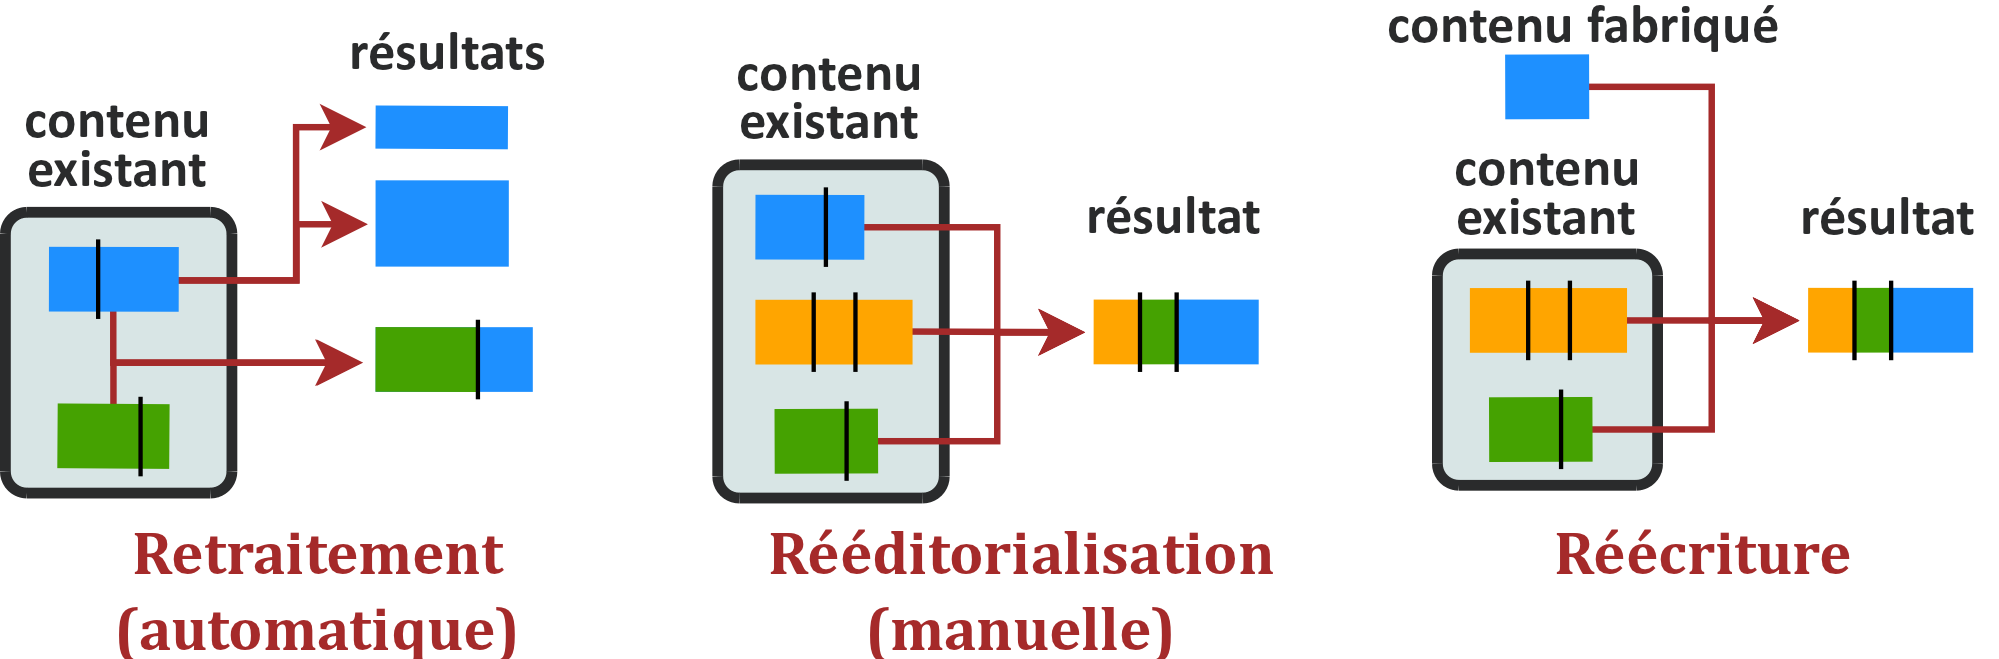
\includegraphics[width=0.75\textwidth]{images/Reuse-v1.png}
\caption{Les différentes pratiques de réutilisations}
\label{img:intro:reuse}
\end{figure}

Nous proposons donc de définir la terminologie suivante pour distinguer entre trois niveaux successifs de réutilisation, chacun visant à créer un nouveau document mais suivant des opérations différentes (voir Figure \ref{img:intro:reuse}). 
La premier critère distinctif est l'automatisation de la transformation, le second critère repose sur la création originale de contenu plutôt que la réorganisation d'un existant : 
\begin{liste}
	\item le \eg{retraitement} (repurposing) qui se caractérise par une automatisation de la transformation opérée sur le contenu (quelque soit son type), c'est-à-dire que cette transformation est effectué par un logiciel lui-même paramétré par un humain. 
	Ces transformations visent à modifier la forme d'expression du document, extraire des fragments de contenu de différentes sources pour les aggréger dans un nouveau document, ou bien encore réorganiser automatiquement la structure du contenu. 
	Le retraitement dépasse le polymorphisme en ce sens où il est possible de gérer de multiple sources de contenus pour construire dynamiquement un nouveau document. 
	Dans le cas de l'audiovisuel, il s'agit des pratiques de réencodage, de changements de format d'encapsulation etc.
	Pour reprendre l'exemple précédent (\ref{sec:ex-reuse}) d'un contenu TV pour une diffusion Web, ou bien encore la création automatique de résumé de rencontres sportives etc. \\

	\item la \eg{rééditorialisation} (reediting) se caractérise par une transformation (manuelle et automatique) de contenus existants. 
	Le document doit s'adapter à un nouveau contexte de lecture (genre éditoriale, public, forme d'expression etc.).
	La transformation du contenu nécessite une compréhension du nouveau contexte de lecture et consiste en des opérations de réorganisation, de mise en relation avec d'autres contenus, de traduction etc. 
	Ces opérations ne se limitent pas à une transformation de la forme d'expression du document (retraitement) mais ne constituent pas une création originale de contenus (réécriture). 
	Simplement, on réutilise divers contenus existants pour créer un nouveau document.  
	La ré-éditorialisation repose donc sur le polymorphisme et la réutilisation au sens de \cite{Crozat2011}.
	Dans le cas de l'audiovisuel, il s'agit typiquement de pratiques de re-montage et de nouvelles sélections de contenu. 
	Pour reprendre l'exemple précédent, il s'agit de monter différemment une séquence initialement prévue pour un journal TV et qui doit s'insérer dans un DVD etc. \\

	 
	\item la \eg{réécriture} (reauthoring) se caractérise par une transformation de contenus existants accompagnée d'une création de contenu original. 
	L'ajout de contenu sert à satisfaire soit aux attentes spécifiques du nouveau public cible, aux contraintes d'un nouveau genre éditorial (commentaires, explications, exemples etc.) soit à la création d'une version augmentée d'un document existant (pas de changement de public cible, mais de nouvelles attentes).
	Dans le cas de l'audiovisuel, il s'agit par exemple de la construction d'un documentaire à partir de vidéo d'archives, la création originale étant le commentaire proposé.\\	 
\end{liste}

Les pratiques de réutilisations sont donc chevillées aux dimensions techniques, éditoriales et sémiotiques du contenu audiovisuel. 
Leur mise en place pose également des problèmes dans l'organisation de la chaîne de production audiovisuelle et son informatisation
% Il faut donc élargir le champ de la modélisation des contenus à une dimension sémiotique et éditoriale et faire le lien avec le déroulement de la production.

%%%%%%%%%%%%%%%%%%%%%%%%%%%%%%%%%%%%%%%%%%%%%%%
\subsection{Évolutions de la chaîne de production (M)}\label{sec:rechaine}
\e{
Les changements introduits par la réutilisation dans la chaîne de production sont donc plus vastes qu'une simple adaptation technique à de nouveaux modes de distribution. %(canal de diffusion + terminal de lecture). 
Il s'agit également de prendre en compte l'audience visée pour affiner encore plus l'adaptation du contenu à ses futurs consomateurs/lecteurs.
L'objectif est de favoriser le développement de variantes d'un même programme soit par la restructuration du contenu (retraitement ou rééditorialisation) ou par l'ajout de contenus (réécriture). 
L'introduction d'acteurs tiers dans une chaîne de production pour fabriquer ou fournir du contenu ne peut se faire sans une plus grande maîtrise des contenus et une meilleure description de ces derniers dès la pré-production.
En effet, le client qui souhaite déléguer la fabrication de contenu à un fournisseur tiers doit d'abord définir ses attentes. 
À l'inverse, si le fournisseur connaît son contenu le client lui a besoin d'un descriptif pour sélectionner les fragments les plus pertinents.
Ainsi, les chaînes de production des clients et des fournisseurs doivent évoluer pour gérer (fournir/acquérir) non pas juste du contenu, mais des descriptions (adjointes ou pas à du contenu) facilitant le travail de leurs partenaires (fabrication ou réutilisation).
}
% Le producteur-diffuseur rentre alors dans une dynamique d'adaptation de ces contenus.

Comme nous l'avons constaté en \ref{sec:electro}, le développement de l'électronique offre de nouvelles opportunités de production mixte, soit avec des amateurs, soit avec d'autres professionnels. 
Cependant, une organisation souhaitant profiter de ces opportunités devra réussir d'abord à encadrer ses partenaires et clarifier avec eux les termes de leurs accords. 
Ce qui auparavant pouvait se résoudre \e{de visu} ou de manière informelle doit maintenant être explicité afin de clarifier la demande, c'est-à-dire le contenu souhaité. 
Qu'il s'agisse de passer commande, ou bien de rechercher dans des bases existantes, cette étape s'apparente à la définition du besoin, à l'écriture d'un cahier des charges, ou dans les termes propres à la production audiovisuelle, au \e{Scripting} défini en \ref{sec:preprod}. 
Maintenant que la fabrication du contenu est déléguée à des tiers, il reste cependant à récupérer le résultat et à vérifier qu'il satisfait à la demande initiale. 
Cette dernière étape nommée généralement \e{Acquisition} constitue un travail à part entière puisqu'il s'agit de \gui{faire rentrer} le contenu dans les \gui{cases} du système d'information et de gestion des contenus. 
En plus des questions de formats informatiques, s'ajoute souvent le problème de la description des contenus et de leur classification en vue de leur utilisation future.  
L'acquisition dépend grandement des conventions établies avec le fabricant/livreur de contenu et impacte directement sur le temps passé à faire le \e{derushing}. 

Côté client, on transforme d'abord la phase de scripting en l'expression d'une \pc{Commande} ou d'une \pc{Requête} ce qui permet de déléguer la fabrication des contenus à un tiers.
Ensuite, on vérifie par \pc{Acquisition} du contenu que le résultat correspond bien à la demande et on procède aux ajustements nécessaires (si besoin) pour satisfaire aux contraintes de notre système (voir Figure \ref{img:intro:evochain}). 

\begin{figure}[ht!]
\centering
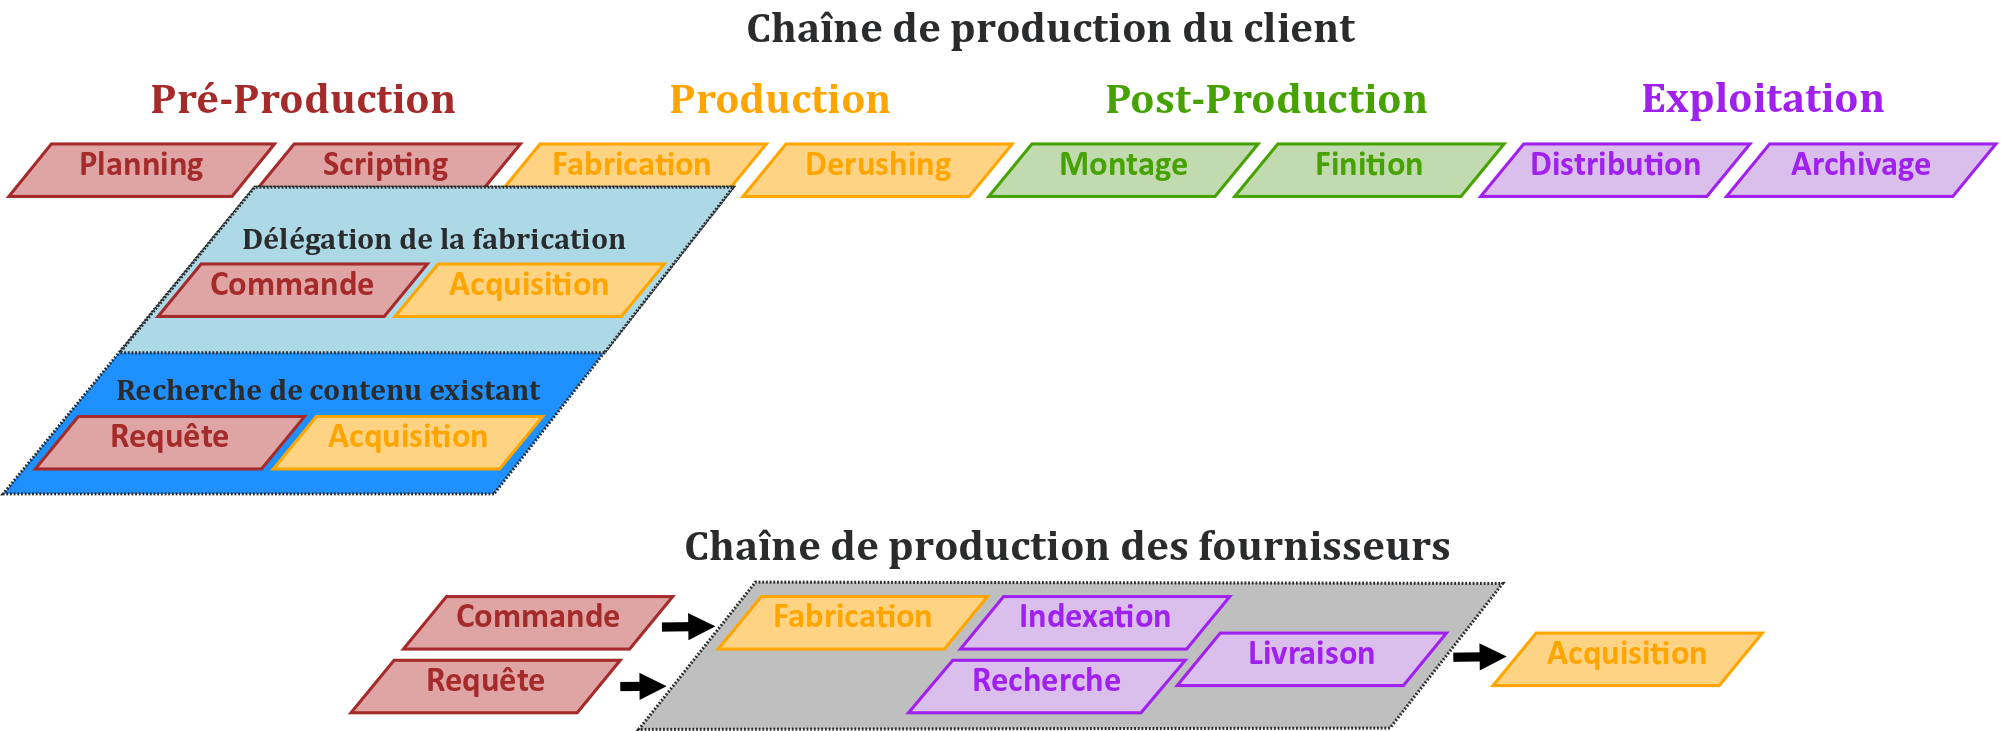
\includegraphics[width=\textwidth]{images/Workflow-Thesis-v6.png}
\caption{Ouverture des chaînes de production du client et du fournisseur}
\label{img:intro:evochain}
\end{figure}

Du côté des fournisseurs de contenu, il existe une distinction entre les chaînes du fabricant et du fournisseur du contenu :  

\begin{liste}
	\item \e{déléguer la fabrication à des contributeurs tiers} : l'utilisation du scripting pour définir la \pc{Commande} de contenu attendu semble une solution satisfaisante, à condition que le vocabulaire utilisé soit normé et rattaché à une conceptualisation de manière à éviter la confusion ou les différences d'interprétations. 
    Lorsqu'il s'agit d'amateurs, la situation se complique car on ne peut pas s'appuyer sur une conceptualisation commune de la production audiovisuelle pour clarifier la commande. 
    De plus, le manque d'expérience et l'ignorance des usages du métier impliquent non seulement de documenter les concepts par des mots et des définitions, mais aussi d'expliquer ce qu'il faut faire durant la phase de \pc{Fabrication}. 
    En d'autres termes, en travaillant avec des amateurs, les professionnels ne se retrouvent non pas à écarter la confusion entre des mots se reférant au même concept, mais à expliquer les opérations auxquelles ces concepts font référence. 
    De même pour l'acquisition, s'il s'agit surtout de se mettre d'accord entre professionnels, travailler avec des amateurs semble plus difficile de prime abord. 
    Les notions de formats d'encodage et d'encapsulation sont souvent confuses ou se mélangent, de même que la description des contenus peut s'avérer compliquée à réaliser sans expérience préalable. 
    Tout du moins, il faut remarquer que la description de la demande initiale sert de description a minima du contenu produit, même si les variations ou les écarts ne sont pas forcément indiqués.
    Le cas échéant, une phase d'\pc{Indexation} peut être nécessaire pour décrire le contenu suivant les exigences du client.\\

	\item \e{rechercher des contenus existants depuis les bases professionnelles} : l'utilisation du vocabulaire de l'écriture audiovisuelle pour définir une \pc{Requête} nécessite une indexation utilisant ce même vocabulaire, ou alors une manière de traduire la requête d'un langage à l'autre (par alignement des vocabulaires par exemple). 
	De même, il faut pouvoir s'accorder sur le niveau de fragmentation recherché (programme complet, séquences, scène, frame etc.), le format du contenu, les descriptions ou les métadonnées à fournir etc.
	Ainsi, la \pc{Livraison} de contenu ne consiste pas en un simple transfert de fichier, mais représente le moment où l'on teste l'interopérabilité entre les systèmes et les formats. 
	Cette étape est d'autant plus cruciale qu'elle se répercute directement sur la phase d'acquisition pour le client. 
	Tout ce qui n'a pas pu être résolu à la livraison (côté fournisseur) devra l'être au moment de l'acquisition dans le système (côté client).\\
	% un vocabulaire de requêtes, s'accorder sur les niveaux de fragmentation, le format de livraison, le contenu de la livraison
\end{liste}



Finalement, il nous faut encore éclairer à quels moments dans la chaîne de production les différentes pratiques de réutilisation sont réalisées (voir définition en \ref{sec:reuse}).
De manière générale, on considère que la réutilisation commence à la phase de pré-production, au moment du \pc{Planning} et du \pc{Scripting} où l'on spécifie les nouvelles formes et formats d'exploitation (voir Figure \ref{img:intro:reutilisation}). 
Mais chaque pratique opére à différents étapes de la chaîne :
\begin{liste}
	\item pour le \e{retraitement}, les variations sur la forme d'expression du document se réalisent en phase de \pc{Finition}. 
	C'est à ce moment que l'original et les variantes sont encodés et encapsulés dans les formats correspondants à leur mode de distribution. 
	Lorsqu'il y a manipulation de la structure des contenus, ces opérations (automatisées) se réalisent à la phase de \pc{Montage}.

	\item pour la \e{rééditorialisation}, le travail commence en phase de \pc{Derushing}, par la sélection des séquences de contenu à ajouter ou à retirer du contenu original. 
	La grande différence avec le retraitement, c'est que cette sélection s'effectue manuellement sur les contenus à disposition. 
	Ensuite, on opére un nouveau \pc{Montage} qui peut également impliquer une \pc{Finition} différente.

	\item pour la \e{réécriture}, la grande différence avec les autres pratiques est que l'on ajoute une nouvelle phase de \pc{Fabrication}. 
	Qu'il s'agisse de création originale ou de récupération de contenu chez un fournisseur tiers, la réécriture consiste à utiliser de nouveaux contenus. 
	Ensuite, on sélectionne en \pc{Derushing} les séquences qui permettront de réaliser un nouveau \pc{Montage}. 
	Finalement, plusieurs \pc{Finition} sont à envisager suivant les cas d'exploitation.
\end{liste}
% conséquences de la réutilisation dans la chaîne : à quel étape ça se joue

\begin{figure}[ht!]
\centering
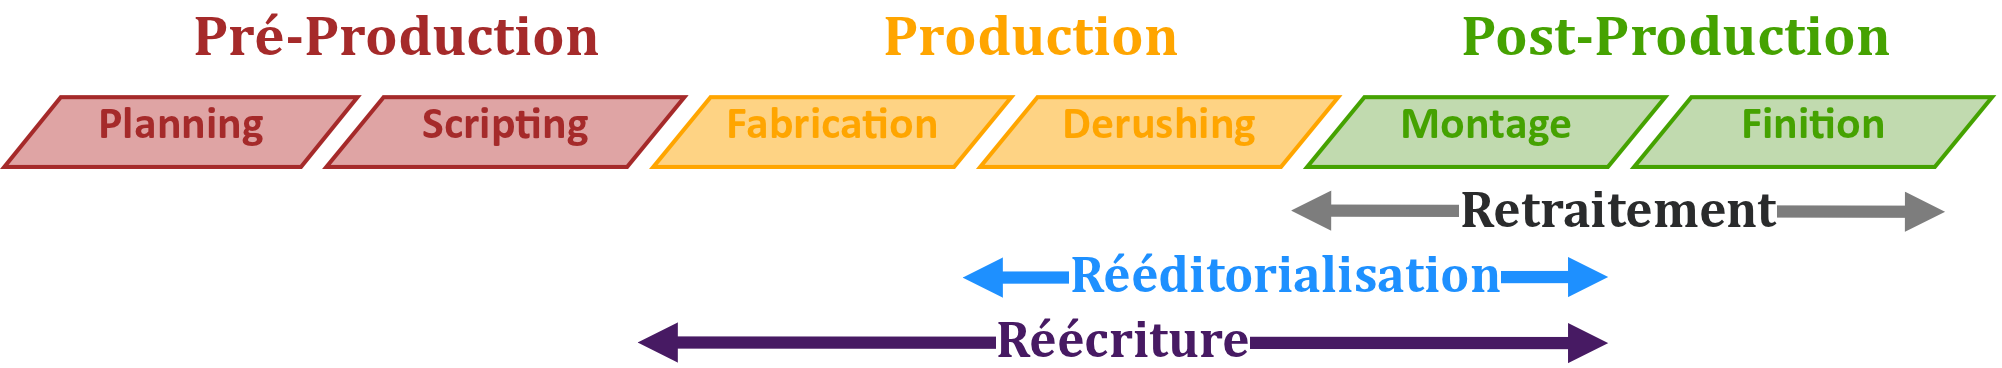
\includegraphics[width=0.8\textwidth]{images/Workflow-Reuse-v1.png}
\caption{Les différentes formes de réutilisation et leur mise en oeuvre dans la chaîne de production audiovisuelle.}
\label{img:intro:reutilisation}
\end{figure}
